\documentclass[
11pt, % The default document font size, options: 10pt, 11pt, 12pt
%codirector, % Uncomment to add a codirector to the title page
]{charter} 


% El títulos de la memoria, se usa en la carátula y se puede usar el cualquier lugar del documento con el comando \ttitle
\titulo{Desarrollo de hardware y firmware para un sistema de control, gestión y comunicación de luminaria pública} 

% Nombre del posgrado, se usa en la carátula y se puede usar el cualquier lugar del documento con el comando \degreename
\posgrado{Carrera de Especialización en Sistemas Embebidos} 
%\posgrado{Carrera de Especialización en Internet de las Cosas} 
%\posgrado{Carrera de Especialización en Inteligencia Artificial}
%\posgrado{Maestría en Sistemas Embebidos} 
%\posgrado{Maestría en Internet de las cosas}
% IMPORTANTE: no omitir titulaciones ni tildación en los nombres, también se recomienda escribir los nombres completos (tal cual los tienen en su documento)
% Tu nombre, se puede usar el cualquier lugar del documento con el comando \authorname
\autor{Ing. Juan Manuel Guariste}

% El nombre del director y co-director, se puede usar el cualquier lugar del documento con el comando \supname y \cosupname y \pertesupname y \pertecosupname
\director{Ing. Juan Manuel Cruz}
\pertenenciaDirector{FIUBA} 
\codirector{} % para que aparezca en la portada se debe descomentar la opción codirector en los parámetros de documentclass
%\pertenenciaCoDirector{FIUBA}

% Nombre del cliente, quien va a aprobar los resultados del proyecto, se puede usar con el comando \clientename y \empclientename
\cliente{Ing. Bernardo Martínez Sáenz}
\empresaCliente{Deitres S.A.}
 
\fechaINICIO{20 de agosto de 2024}		%Fecha de inicio de la cursada de GdP \fechaInicioName
\fechaFINALPlan{8 de octubre de 2024} 	%Fecha de final de cursada de GdP
\fechaFINALTrabajo{junio de 2025}	%Fecha de defensa pública del trabajo final


\begin{document}

\maketitle
\thispagestyle{empty}
\pagebreak


\thispagestyle{empty}
{\setlength{\parskip}{0pt}
\tableofcontents{}
}
\pagebreak


\section*{Registros de cambios}
\label{sec:registro}


\begin{table}[ht]
\label{tab:registro}
\centering
\begin{tabularx}{\linewidth}{@{}|c|X|c|@{}}
\hline
\rowcolor[HTML]{C0C0C0} 
Revisión & \multicolumn{1}{c|}{\cellcolor[HTML]{C0C0C0}Detalles de los cambios realizados} & Fecha      \\ \hline
0      & Creación del documento                                 &\fechaInicioName \\ \hline
1      & Se completa hasta el punto 5 inclusive           & 3 de septiembre de 2024 \\ \hline
2      & Se completa hasta el punto 9 inclusive	       & 10 de septiembre de 2024 \\ \hline
%		  Se puede agregar algo más \newline
%		  En distintas líneas \newline
%		  Así                                                    & {día} de {mes} de 202X \\ \hline
3      & Se completa hasta el punto 12 inclusive                & 17 de septiembre de 2024 \\ \hline
4      & Se completa hasta el punto 15 inclusive	                                 & 24 de septiembre de 2024 \\ \hline
5      & Se aplican correcciones	                                 & 26 de septiembre de 2024 \\ \hline

% Si hay más correcciones pasada la versión 4 también se deben especificar acá

\end{tabularx}
\end{table}

\pagebreak



\section*{Acta de constitución del proyecto}
\label{sec:acta}

\begin{flushright}
Buenos Aires, \fechaInicioName
\end{flushright}

\vspace{2cm}

%Por medio de la presente se acuerda con el \authorname\hspace{1px} que su Trabajo Final de la \degreename\hspace{1px} se titulará ``\ttitle'' y consistirá en \textcolor{red}{la implementación de un prototipo de un sistema de control de temperatura de una caldera industrial}. El trabajo tendrá un presupuesto preliminar estimado de \textcolor{red}{600} horas y un costo estimado de \textcolor{red}{U\$D 1000}, con fecha de inicio el \fechaInicioName\hspace{1px} y fecha de presentación pública el \fechaFinalName.

%Se adjunta a esta acta la planificación inicial.

Por medio de la presente se acuerda con el \authorname\hspace{1px} que su Trabajo Final de la \degreename\hspace{1px} se titulará ``\ttitle'' y consistirá en la implementación de un prototipo para el control eficiente y remoto de las luminarias, permitiendo una comunicación efectiva y robusta entre ellas y una gestión centralizada. El trabajo tendrá un presupuesto preliminar estimado de 634 horas y un costo estimado de USD 10993, con fecha de inicio el \fechaInicioName\hspace{1px} y fecha de presentación pública en \fechaFinalName.

Se adjunta a esta acta la planificación inicial.

\vfill

% Esta parte se construye sola con la información que hayan cargado en el preámbulo del documento y no debe modificarla
\begin{table}[ht]
\centering
\begin{tabular}{ccc}
\begin{tabular}[c]{@{}c@{}}Dr. Ing. Ariel Lutenberg \\ Director posgrado FIUBA\end{tabular} & \hspace{2cm} & \begin{tabular}[c]{@{}c@{}}\clientename \\ \empclientename \end{tabular} \vspace{2.5cm} \\ 
\multicolumn{3}{c}{\begin{tabular}[c]{@{}c@{}} \supname \\ Director del Trabajo Final\end{tabular}} \vspace{2.5cm} \\
\end{tabular}
\end{table}

\section{1. Descripción técnica-conceptual del proyecto a realizar}
\label{sec:descripcion}

El proyecto está alineado con las necesidades de Deitres S.A., empresa donde el autor de este proyecto trabaja como ingeniero de desarrollo de hardware y firmware. Deitres S.A. se especializa en crear soluciones tecnológicas e innovadoras para la seguridad electrónica, domótica y la industria. Este proyecto aborda la ineficiencia en la gestión de la iluminación pública, un problema crítico en las ciudades modernas donde el control efectivo y el ahorro energético son esenciales. Muchas ciudades enfrentan dificultades para mantener un control preciso sobre sus redes de iluminación pública, lo que genera altos costos operativos, de mantenimiento y de consumo energético.

Actualmente, existen diversas soluciones para la gestión de la iluminación pública, desde sistemas básicos de encendido y apagado programado hasta tecnologías más avanzadas que permiten el control remoto y la automatización. Sin embargo, muchas de estas soluciones tienen limitaciones en términos de escalabilidad, robustez de comunicación y capacidad de integración con otras tecnologías.

La solución propuesta es el CityLight, un prototipo de luminaria inteligente que se conecta a Internet a través de Wi-Fi y redes celulares. Estos dispositivos, una vez instalados, interactúan entre sí formando una red con topología mesh en 915 MHz, utilizando un protocolo propio desarrollado por la empresa e implementado en otros de sus productos. Si un dispositivo necesita comunicar un evento o el estado de una luminaria y no cuenta con conexión a Internet, podrá utilizar esta red mesh para conectarse con otro CityLight que funcione como gateway. Esto no solo garantiza un sistema de comunicación eficiente y robusto, sino que también ofrece la ventaja de superar una eventual obsolescencia tecnológica. Por ejemplo, si en una ciudad se desmantelan las redes celulares 3G, los CityLight que utilizaban esa interfaz de conexión a Internet podrán seguir comunicando sus eventos a través de la red mesh, conectándose a otros CityLight con otras formas de conexión, como Wi-Fi. Además, si surge una nueva tecnología de conexión a Internet, como la satelital o 5G, bastará con que un solo CityLight disponga de esa interfaz para que pueda actuar como gateway para los demás nodos de la red mesh.

A continuación, se detallan las funcionalidades específicas que se implementarán en el prototipo de luminaria inteligente, CityLight:

\begin{itemize}
		\item \textbf{Conector NEMA:} dispondrá de una interfaz física NEMA para conectarse a las luminarias, permitiendo una integración estándar con diversos sistemas de iluminación existentes.
        \item \textbf{Medición de intensidad lumínica ambiental mediante sensor fotosensible (fotocélula)}: permitirá ajustar la iluminación en función de las condiciones de luz externa.
        \item \textbf{Actuación sobre la intensidad lumínica de la luminaria mediante circuito dimmer}: facilitará el ajuste de la intensidad de la luz según las necesidades.
        \item \textbf{Medición de consumo de corriente AC}: para monitorear el consumo energético de las luminarias.
        \item \textbf{Detección de presencia de tensión AC}: para asegurar el correcto funcionamiento del sistema.
        \item \textbf{Utilización de circuito adaptador de señales para control de la luminaria}: adaptará las señales de control.
        \item \textbf{Control de habilitación/deshabilitación de suministro de corriente a la luminaria mediante accionamiento de relé}: permitirá encender o apagar las luminarias de manera automatizada o por comandos enviados remotamente.
        \item \textbf{Interfaz de conexión a Internet}: el sistema podrá recibir comandos y enviar reportes a través de interfaces Wi-Fi y celular. Se le podrá consultar el estado de la luminaria y actuar sobre ella.
        \item \textbf{Red mesh}: implementación de la red mesh en 915 MHz que permita la comunicación entre dispositivos CityLight. 
        \item \textbf{Geo-posicionamiento de luminarias}: utilización de GPS para la localización precisa de cada unidad.
        \item \textbf{Posibilidad de operar con alimentación alterna o a batería}:  asegurará la operación del sistema bajo diversas condiciones de suministro energético.
\end{itemize}

En la figura \ref{fig:diagBloquesGeneral}, se presenta un diagrama en bloques del sistema propuesto en el que se observan las distintas funcionalidades a implementar. 

\begin{figure}[htpb]
\centering 
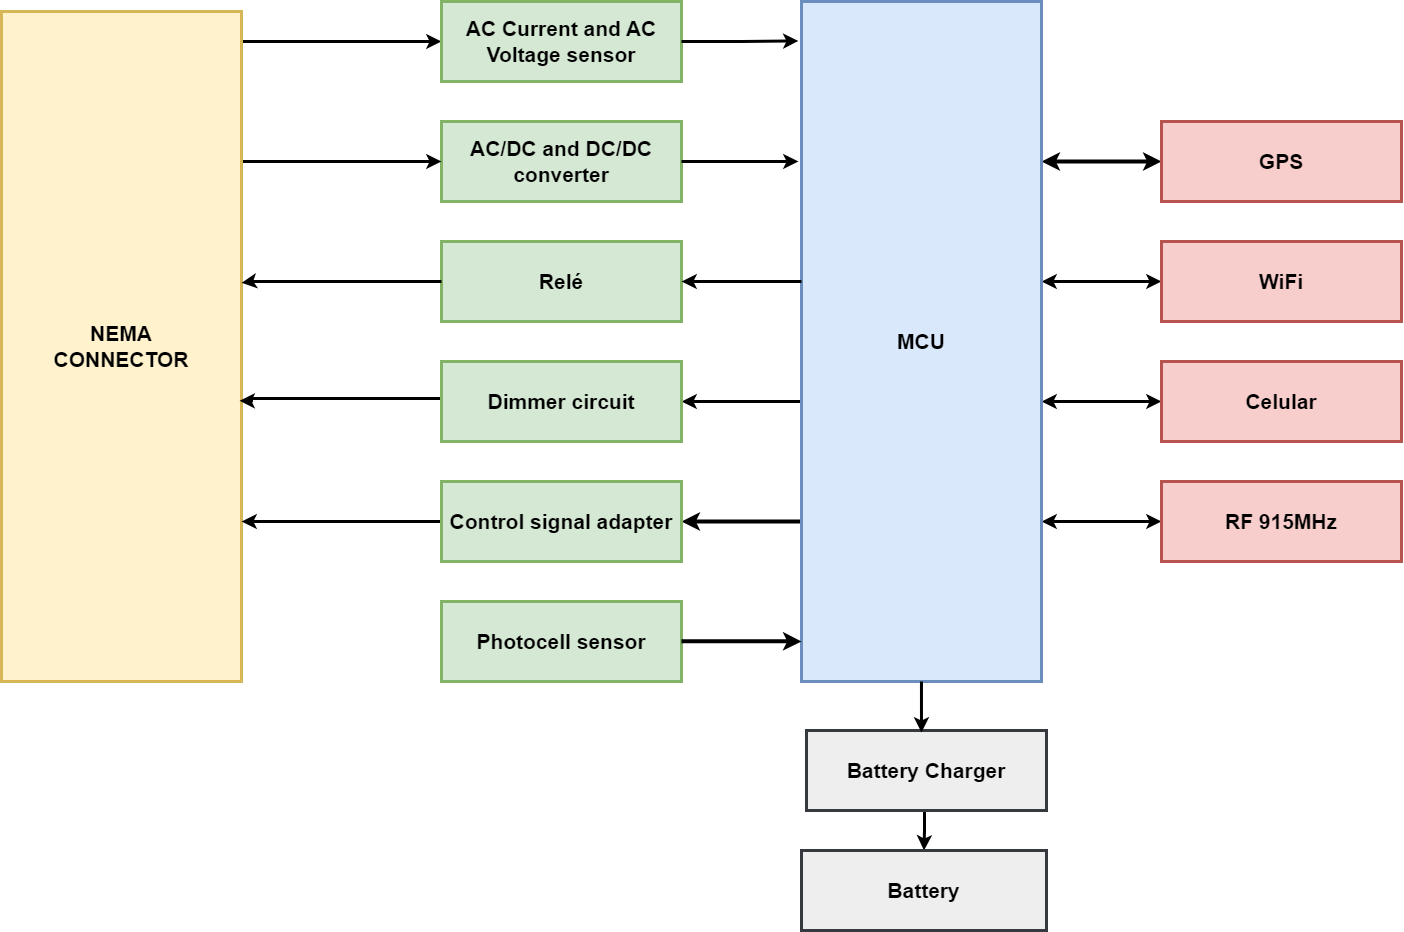
\includegraphics[width=.9\textwidth]{./Figuras/diagBloquesGeneral.png}
\caption{Diagrama en bloques del sistema.}
\label{fig:diagBloquesGeneral}
\end{figure}

El cliente de este proyecto valora la aplicación de la red mesh en 915 MHz debido a su éxito en otros productos desarrollados por la empresa. La integración de esta red distingue al proyecto CityLight de otras soluciones, ofreciendo una comunicación más robusta y eficiente entre las luminarias y mejorando la escalabilidad del sistema. Este proyecto es crucial para Deitres S.A. porque permitirá expandir el uso de una tecnología ya validada y apreciada, reforzando su posición en el mercado de soluciones para la gestión de infraestructuras urbanas.

 \pagebreak

\section{2. Identificación y análisis de los interesados}
\label{sec:interesados}

\begin{table}[ht]
%\caption{Identificación de los interesados}
%\label{tab:interesados}
\begin{tabularx}{\linewidth}{@{}|l|X|X|p{5cm}|@{}}
\hline
\rowcolor[HTML]{C0C0C0} 
Rol           & Nombre y Apellido & Organización 	& Puesto 	\\ \hline
%Auspiciante   &                   &              	&        	\\ \hline
Cliente       & \clientename      &\empclientename	&CEO de Deitres S.A.      	\\ \hline
%Impulsor      &                   &              	&        	\\ \hline
Responsable   & \authorname       & FIUBA        	& Alumno 	\\ \hline
Colaboradores &       Gustavo Vasoin  \newline Ing. Daniel Alejandro Ismael          &      Deitres S.A.  \newline Deitres S.A. 	&   Desarrollador de firmware \newline  Desarrollador de hardware y firmware\\ \hline
Orientador    & \supname	      & \pertesupname 	& Director del Trabajo Final \\ \hline
%Equipo        & miembro1 \newline 
%				miembro2          &              	&        	\\ \hline
%Opositores    &                   &              	&        	\\ \hline
Usuario final &Municipalidades y empresas de infraestructura urbana         &-              	&-        	\\ \hline
\end{tabularx}
\end{table}

Cliente: el Ing. Bernardo Martínez Sáenz es un líder con amplia experiencia en el sector de la seguridad electrónica y la domótica. Su visión estratégica en la implementación de soluciones innovadoras será fundamental para guiar el desarrollo del proyecto CityLight.

Orientador: el Ing. Juan Manuel Cruz es un profesional de alta capacidad técnica y de gestión, con una destacada trayectoria en el ámbito de sistemas embebidos. Sus observaciones y recomendaciones serán fundamentales para el éxito del proyecto, ya que aportará no solo su experiencia técnica, sino también su visión estratégica para guiar el desarrollo y asegurar que se alcancen los objetivos propuestos.

Colaboradores: Gustavo Vasoin es un profesional con una sólida trayectoria en el desarrollo de firmware para sistemas embebidos. El Ing. Daniel Alejandro Ismael, con amplia experiencia en el  diseño y desarrollo de hardware y firmware, aporta un enfoque integral en la creación de sistemas electrónicos. Ambos trabajan en la empresa para la cual se desarrolla el producto. Su experiencia y conocimientos técnicos serán fundamentales para lograr un producto de alta calidad, cumpliendo con los estándares de innovación y eficiencia que demanda el proyecto.

\section{3. Propósito del proyecto}
\label{sec:proposito}

Mejorar la eficiencia en la gestión de la iluminación pública, reducir los costos operativos y de mantenimiento, y optimizar el consumo energético. Se busca desarrollar un sistema de luminarias inteligentes con conexión a Internet que permita un control preciso y remoto, garantizando una comunicación robusta y escalable entre las luminarias mediante una red mesh.

\pagebreak

\section{4. Alcance del proyecto}
\label{sec:alcance}

El proyecto incluye el diseño de circuito impreso y desarrollo de firmware que permita:
\begin{itemize}
	\item Conexión con el conector NEMA.
	\item Adquisición de señales y control de la luminaria.
	\item Implementar interfaces de conexión a Internet mediante Wi-Fi y red celular.
	\item Geolocalización mediante modulo GPS.
	\item Implementación de red mesh en 915 MHz.
	\item Integración del CityLight con el software de control y gestión existente en la empresa.
\end{itemize}	

El proyecto no incluye:
\begin{itemize}
	\item Desarrollo de nuevo software de control y gestión para los dispositivos.
	\item Pruebas de campo del prototipo.
	\item Certificación del prototipo ante organismos regulatorios nacionales y/o internacionales.
\end{itemize}


\section{5. Supuestos del proyecto}
\label{sec:supuestos}


Para el desarrollo del presente proyecto se supone que: 

\begin{itemize}
	\item El Ing. Juan Manuel Guariste, responsable del proyecto, y el Ing. Bernardo Martínez Sáenz, cliente del proyecto, estan de acuerdo con los requerimientos y 		alcance planteado en este documento.
	\item El presupuesto necesario para el desarrollo estará a cargo de la empresa Deitres S. A.
	\item El Ing. Juan Manuel Guariste dispondrá eventualmente de tiempo de la jornada laboral para llevar a cabo el proyecto en el plazo especificado en el acta de constitución.
	\item Se conseguirán todos los componentes necesarios para el desarrollo en tiempo y forma.	
	%\item Se dispondrá del instrumental de laboratorio adecuado para realizar mediciones al prototipo.
	\item En caso de no contar con algún conocimiento específico para desarrollar el proyecto, se podrá contar con el apoyo o soporte del cuerpo docente de la especialización.
\end{itemize}

\pagebreak

\section{6. Requerimientos}
\label{sec:requerimientos}

\begin{enumerate}
	\item Requerimientos asociados con el hardware:
		\begin{enumerate}
			\item El sistema debe contar con una interfaz física NEMA de 7 pines para conectarse y comunicarse con las luminarias de alumbrado público.
			\item La implementación debe ser compatible con una carcasa genérica para luminarias. En caso de ser necesario, se debe permitir el montaje de un PCB encima de otro para optimizar el uso del espacio disponible y facilitar la integración de todos los componentes.
			\item  El sistema debe integrar un sensor de efecto Hall para medir el consumo de corriente AC de la luminaria conectada.
			\item El sistema debe integrar un optoacoplador para detectar la presencia de tensión AC en la luminaria.
 			\item El sistema debe integrar un circuito dimmer que sea capaz de regular la intensidad lumínica de la luminaria.
			\item Debe contar con un sensor fotosensible que mida la intensidad lumínica ambiental.
			%\item Debe poseer circuitería de adaptación de señales de control.
			\item El sistema debe integrar un relé que sea controlado por el microcontrolador y que permita habilitar o deshabilitar el suministro de corriente a la luminaria.
			\item Debe integrar un módulo Wi-Fi para la conectividad a Internet.
			\item Debe integrar un módulo celular para la conectividad a Internet.
			\item El sistema debe implementar un transceptor en la banda de 915 MHz para establecer y mantener la red mesh de luminarias.
			\item Debe utilizar un amplificador para el transceptor de 915 MHz que permita aumentar la potencia de salida al menos 20 dBm.
			\item El sistema debe incluir un módulo GPS para obtener la posición geográfica de cada luminaria y sincronizar datos como la hora y ubicación precisa.
			\item Debe ser capaz de operar tanto con alimentación de la red eléctrica como a través de una batería en caso de cortes o fallos en el suministro eléctrico. 
			\item La conmutación entre la alimentación de la red eléctrica y la batería debe ser automática mediante circuitos analógicos, garantizando la continuidad sin	intervención manual.
			\item Se debe implementar un circuito de carga de batería que permita su recarga segura cuando el sistema esté conectado a la red eléctrica.
			\item Se deben implementar circuitos de adaptación para medir señales con el ADC del microcontrolador de manera segura.
			\item El sistema debe ser diseñado con una configuración modular que permita la fabricación de algunos dispositivos CityLight sin los componentes de conexión a Internet, como los módulos de celular y Wi-Fi, y sus circuitos relacionados. Estos dispositivos se comunicarán únicamente a través de la red mesh con un gateway, lo que reducirá significativamente los costos de producción.
		\end{enumerate}

	\item Requerimientos asociados con el firmware:
		\begin{enumerate}		
		\item El firmware debe estar implementado sobre un sistema operativo de tiempo real (RTOS), asegurando el manejo eficiente de múltiples tareas críticas como control, monitoreo y comunicación.
		\item Se debe implementar el protocolo de comunicación para la red mesh utilizando el transceptor de 915 MHz.
		\item EL sistema debe implementar la interfaz de conexión a Internet a través del módulo Wi-Fi, permitiendo al sistema enviar y recibir datos desde plataformas de	gestión remota.
		\item Debe implementar la interfaz de conexión a Internet a través del módulo celular, permitiendo al sistema enviar y recibir datos desde plataformas de gestión remota.
		\item El firmware debe incluir la lógica de selección de conexión a Internet, priorizando la interfaz Wi-Fi cuando ambas conexiones estén disponibles, y conmutando
			 a celular en caso de fallo.
		\item En caso de no disponer conexión a Internet, el sistema debe utilizar la red mesh para comunicarse con un gateway presente en la red, que será el encargado
			 de enviar y recibir datos hacia y desde Internet. 
		\item El firmware debe procesar y gestionar los datos proporcionados por el sensor fotosensible.
		\item El sistema debe permitir el encendido automático de las luminarias según los niveles de luz ambiental detectados, o mediante comandos remotos.
		\item Debe ser posible la actualización del firmware \textit{over-the-air} (OTA).
		\item El firmware debe controlar la intensidad lumínica de las luminarias, regulando la tensión de entrada del circuito dimmer.
		\item El firmware debe procesar la información del módulo GPS para geoposicionamiento y sincronización horaria.
		\item Se deben leer, procesar e informar los datos de consumo eléctrico enviados por el sensor de efecto Hall.
		\item El firmware debe procesar los datos enviados por el optoacoplador para detectar la presencia o ausencia de tensión alterna en la luminaria.
		\item Debe medir y reportar la tensión de la batería utilizando el ADC del microcontrolador.
		\end{enumerate}
\end{enumerate}

\section{7. Historias de usuarios (\textit{Product backlog})}
\label{sec:backlog}

En esta sección se presentan algunas historias de usuarios valoradas en un sistema basado en la estimación de tres categorías: dificultad, complejidad y riesgo o incertidumbre asociadas a cada historia. Para determinar los \textit{story points} de una historia de usuario, se asignaron valores a cada uno de
los siguientes aspectos:

\begin{table}[htpb]
\centering
\begin{tabularx}{\linewidth}{|X|c|c|c|}
\hline
\rowcolor[HTML]{C0C0C0} 
\textbf{Grado} &
\textbf{Dificultad} &
\textbf{Complejidad} &
\textbf{Riesgo o Incertidumbre} \\ \hline
Bajo  &
 1&
 1 &
 2
\\ \hline
Medio  &
 3&
 5&
 3
 \\ \hline
Alto &
 5 &
 13 &
 5
\\ \hline
\end{tabularx}
%\caption{Grados de Dificultad, Complejidad y Riesgo para las historias de usuarios}
\end{table}
Para calcular los \textit{story points}, se suman los valores asignados a cada categoría y el resultado se aproxima al siguiente número de la serie de Fibonacci. Por ejemplo, si la complejidad del trabajo es media (5), la dificultad es baja (1) y la incertidumbre es alta (5), los \textit{story points} serían 13 (5 + 1 + 5 = 11, que se aproxima al siguiente número de Fibonacci, que es 13).

\begin{enumerate}
\item ``Como cliente del proyecto, quiero que el sistema CityLight permita una gestión centralizada y en tiempo real de todas las luminarias instaladas, para optimizar el mantenimiento y reducir los costos operativos, mejorando la eficiencia del servicio."

\textit{Story points}: 13 (complejidad: 5, dificultad: 5, incertidumbre: 3)

\item ``Como usuario final, quiero que el sistema CityLight utilice la red mesh cuando no haya conexión a Internet, para que los eventos se comuniquen a través de un gateway, asegurando la continuidad del servicio."

\textit{Story points}: 13 (complejidad: 5, dificultad: 3, incertidumbre: 3)

\item ``Como usuario final, quiero poder monitorear el consumo eléctrico y la presencia de tensión de cada luminaria, para asegurarme de que estén operando correctamente y 
optimizar el uso de energía."

\textit{Story points}: 8 (complejidad: 1, dificultad: 3, incertidumbre: 2)

%\item ``Como desarrollador de firmware para CityLight, necesito que el sistema permita una implementación modular y bien documentada, para facilitar la integración del protocolo MESH, el control del relé y las actualizaciones OTA, garantizando un desarrollo eficiente y mantenible a largo plazo."

%\textit{Story points}: 8 (complejidad: 3, dificultad: 3, incertidumbre: 3)

\end{enumerate}



\section{8. Entregables principales del proyecto}
\label{sec:entregables}

\begin{itemize}
	\item Manual de usuario.
	\item Esquemáticos de los circuitos electrónicos.
	\item Diseño del PCB.
	\item Archivos de fabricación del PCB.
	\item Prototipo funcional del CityLight.
	\item Código fuente del firmware.
	\item Informe final.
\end{itemize}

\section{9. Desglose del trabajo en tareas}
\label{sec:wbs}

\begin{enumerate}
\item Planificación del proyecto (30 h)
	\begin{enumerate}
	\item Definición de especificaciones y requerimientos (4 h)
	\item Definición de alcance del proyecto (2 h)
	\item Revisión de viabilidad técnica (2 h)
	\item Generación de diagrama de actividades (4 h)
	\item Generación de diagrama de Gantt (2 h)
	\item Análisis presupuestario del proyecto (2 h)
	\item Definición de riesgos y contingencias  (2 h)
	\item Gestión de calidad (4 h)
	\item Presentación y exposición del proyecto (8 h)
	\end{enumerate}
\item Diseño de hardware (96 h)
	\begin{enumerate}
	\item Análisis, selección y adquisición de componentes (8 h)
	\item Diseño de esquemáticos (32 h)
	\item Optimización del diseño del PCB para montaje en carcasa (8 h)
	\item Diseño del PCB (40 h)
	\item Generación de archivos de fabricación (4 h)
	\item Validación, cotización y pedido de fabricación (4 h)
	\end{enumerate}
\item Validación de hardware del prototipo (20 h)
	\begin{enumerate}
	\item Soldado de componentes que no hayan sido ensamblados por el fabricante (4 h)
	\item Limpieza, validación e inspección de conexiones del PCB (8 h)
	\item Pruebas de integridad eléctrica y aislamiento (8 h)
	\end{enumerate}
\item Desarrollo del firmware (296 h)
	\begin{enumerate}
	\item Implementación del RTOS (8 h)
	\item Implementación del protocolo de comunicación para la red mesh (32 h)
	\item Implementación de interfaz de conexión a Internet por Wi-Fi (32 h)
	\item Implementación de interfaz de conexión a Internet por red celular (32 h)
	\item Implementación de manejador de conexiones a Internet (16 h)
	\item Implementación de la adquisición y gestión de los datos provenientes del sensor fotosensible (16 h)
	\item Implementación de la lógica de control de intensidad lumínica mediante circuito dimmer (16 h)
	\item Implementación del control del relé para habilitación/deshabilitación de la luminaria (16 h)
	\item Implementación de control del módulo GPS (32 h)
	\item Implementación de adquisición y gestion de los datos de consumo eléctrico enviados por el sensor de efecto Hall (16 h)
	\item Implementación de adquisición y gestion del dato de presencia o ausencia de tensión alterna enviado por el optoacoplador (8 h)
	\item Implementación de adquisición y gestión de la tensión de batería (8 h)
	\item Implementación de la actualización OTA del firmware (32 h)
	\item Pruebas unitarias y de integración del firmware (32 h)
	\end{enumerate}
\item \textbf{Validación del sistema} (104 h)
	\begin{enumerate}
	\item Pruebas funcionales del sistema completo (32 h)
	\item Pruebas de comunicación y conectividad (Wi-Fi, celular, mesh) (24 h)
	\item Validación del sistema en diferentes condiciones de operación (24 h)
	\item Ajustes y optimizaciones finales (24 h)
	\end{enumerate}
\item \textbf{Documentación final} (88 h)
	\begin{enumerate}
	\item Elaboración de manual de usuario (24 h)
	\item Elaboración de memoria técnica (32 h)
	\item Revisión de memoria técnica (16 h)
	\item Elaboración de la presentación final (16 h)
	\end{enumerate}
\end{enumerate}

Cantidad total de horas: 634 h.

\pagebreak

\section{10. Diagrama de Activity On Node}
\label{sec:AoN}

En la figura \ref{fig:AoN} se presenta el diagrama \textit{Activity On Node}. Se identifican cinco caminos críticos, todos resaltados con flechas rojas, que indican las actividades que determinan la duración mínima del proyecto. El tiempo total estimado para completar cualquiera de los caminos críticos es de 426 horas.


\begin{figure}[htpb]
\centering 
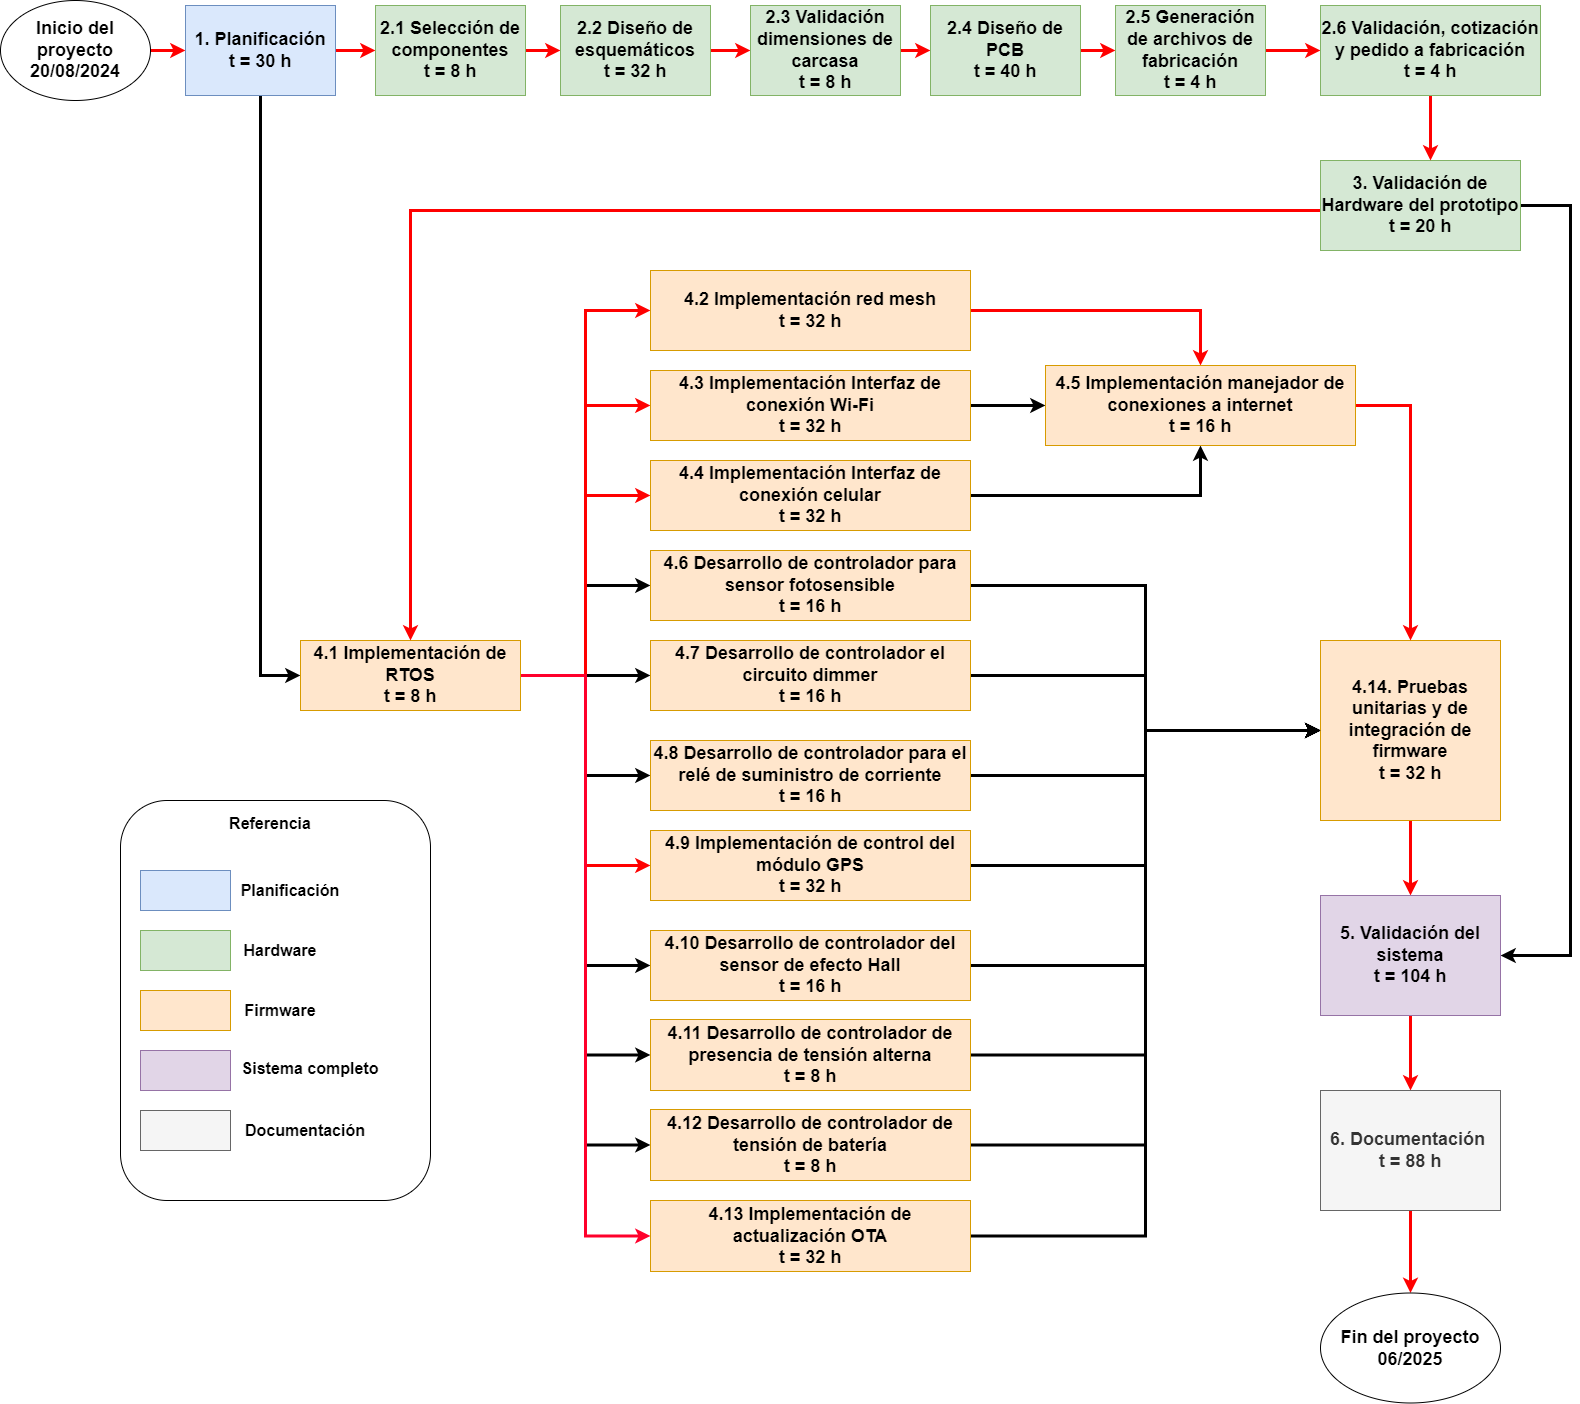
\includegraphics[width=1\textwidth]{./Figuras/AoN.png}
\caption{Diagrama de \textit{Activity on Node}.}
\label{fig:AoN}
\end{figure}

\section{11. Diagrama de Gantt}
\label{sec:gantt}
En las figuras \ref{fig:diagGantt-1} y \ref{fig:diagGantt-2} se muestra el diagrama de Gantt asociado al proyecto.



\begin{landscape}
\begin{figure}[htpb]
\centering 
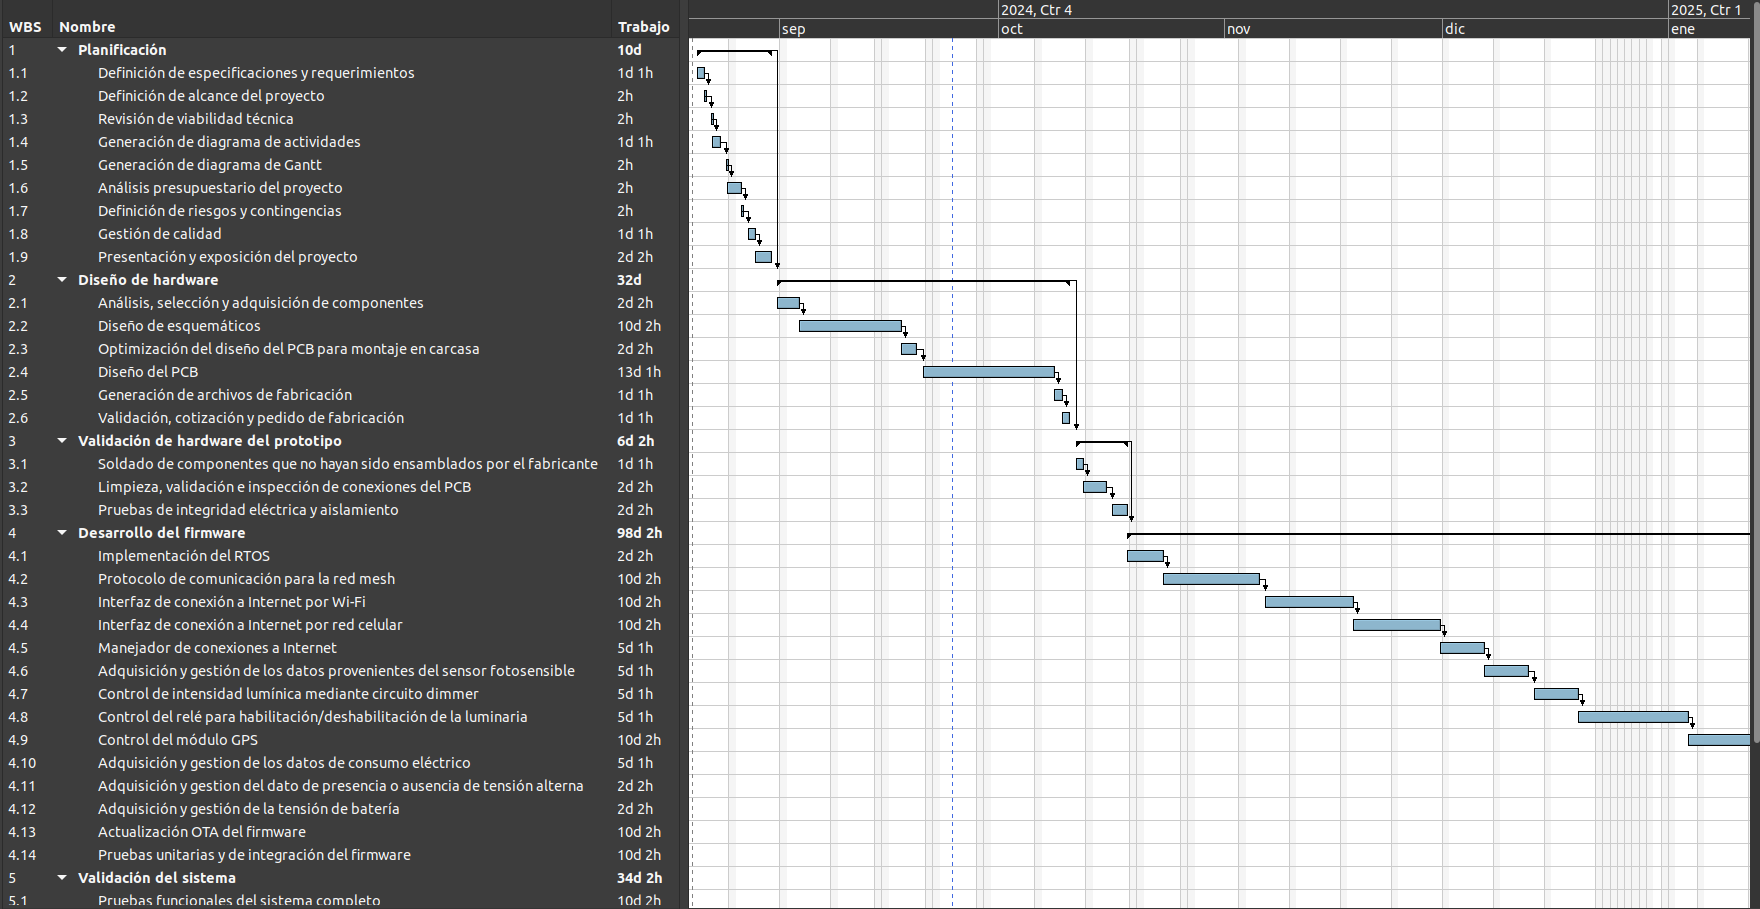
\includegraphics[height=.8\textheight]{./Figuras/Gantt-1.png}
\caption{Diagrama de Gantt (parte 1).} %Modificar este título acorde.
\label{fig:diagGantt-1}
\end{figure}
\end{landscape}

\begin{landscape}
\begin{figure}[htpb]
\centering 
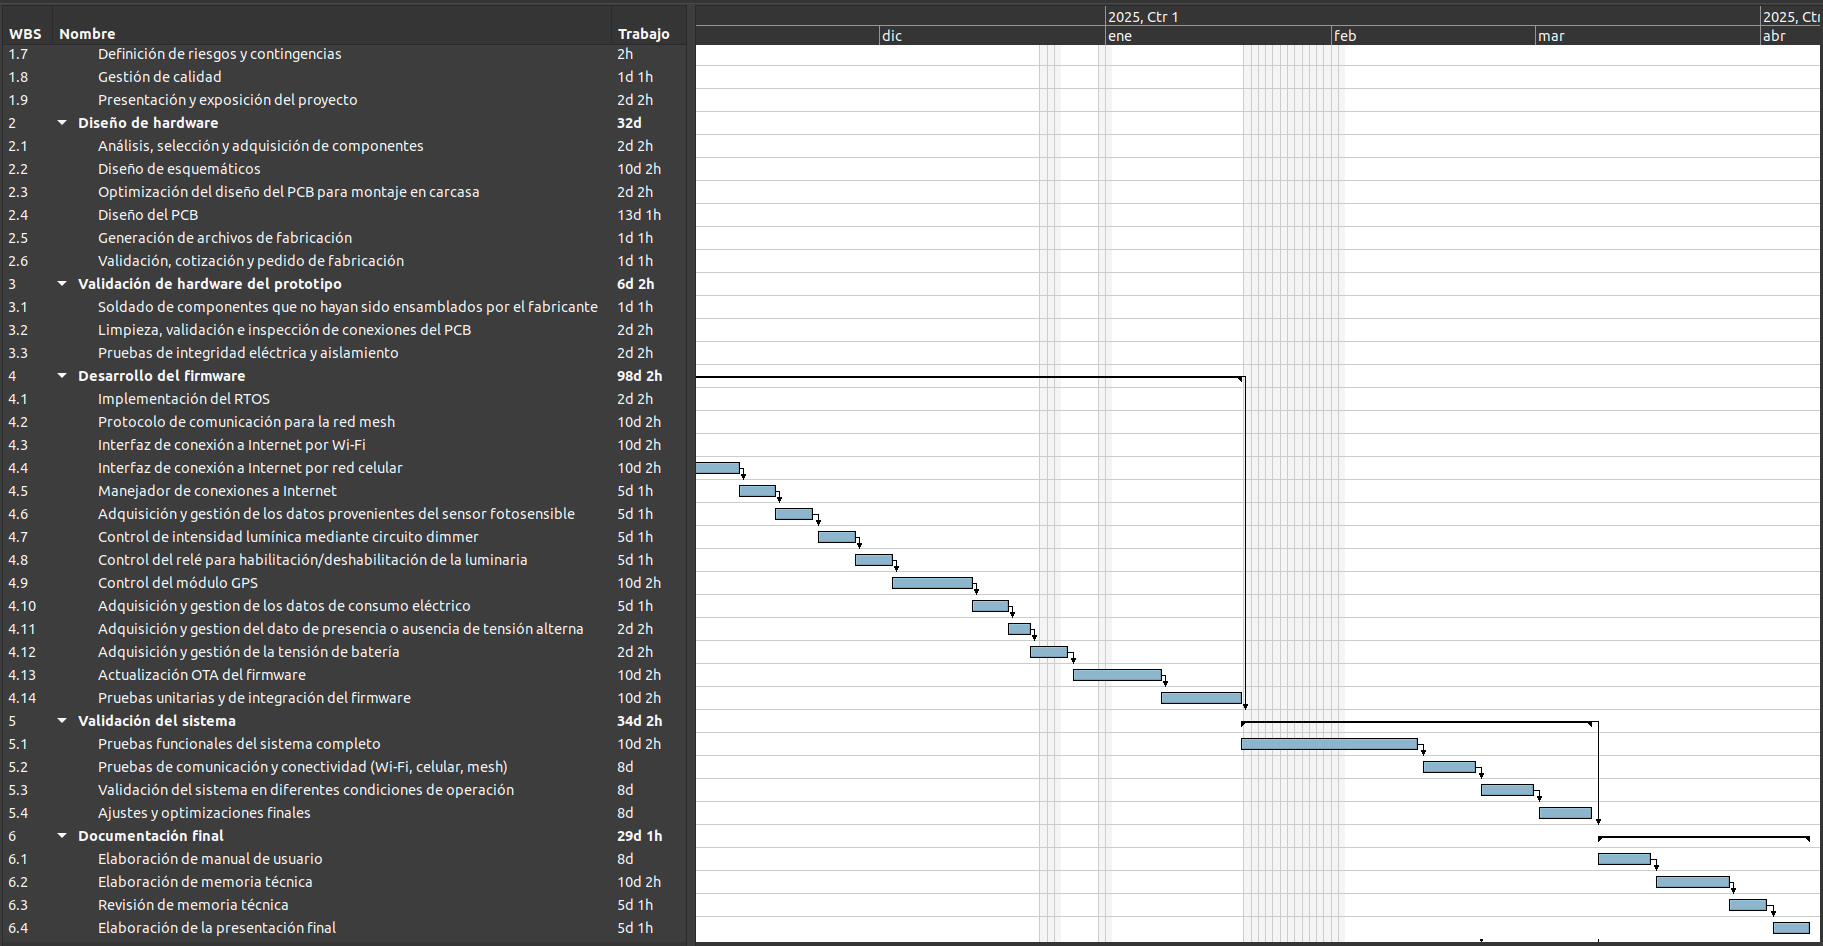
\includegraphics[height=.8\textheight]{./Figuras/Gantt-2.png}
\caption{Diagrama de Gantt (parte 2).} %Modificar este título acorde.
\label{fig:diagGantt-2}
\end{figure}
\end{landscape}


\section{12. Presupuesto detallado del proyecto}
\label{sec:presupuesto}

Los precios presentados en la tabla a continuación están expresados en dólares estadounidenses (USD). La cotización utilizada es de 1 dólar estadounidense equivalente a 962 pesos argentinos (ARS), según el tipo de cambio del 16 de septiembre de 2024.

\begin{table}[htpb]
\centering
\begin{tabularx}{\linewidth}{@{}|X|c|r|r|@{}}
\hline
\rowcolor[HTML]{C0C0C0} 
\multicolumn{4}{|c|}{\cellcolor[HTML]{C0C0C0}COSTOS DIRECTOS} \\ \hline
\rowcolor[HTML]{C0C0C0} 
Descripción &
  \multicolumn{1}{c|}{\cellcolor[HTML]{C0C0C0}Cantidad} &
  \multicolumn{1}{c|}{\cellcolor[HTML]{C0C0C0}Valor unitario} &
  \multicolumn{1}{c|}{\cellcolor[HTML]{C0C0C0}Valor total} \\ \hline
 Componentes electrónicos&
  \multicolumn{1}{c|}{10} &
  \multicolumn{1}{c|}{100} &
  \multicolumn{1}{c|}{1000} \\ \hline
Fabricación del PCB &
  \multicolumn{1}{c|}{10} &
  \multicolumn{1}{c|}{27} &
  \multicolumn{1}{c|}{270} \\ \hline
Horas de ingeniería &
  \multicolumn{1}{c|}{634} &
  \multicolumn{1}{c|}{10} &
  \multicolumn{1}{c|}{6340} \\ \hline
\multicolumn{3}{|c|}{SUBTOTAL} &
  \multicolumn{1}{c|}{7610} \\ \hline
\rowcolor[HTML]{C0C0C0} 
\multicolumn{4}{|c|}{\cellcolor[HTML]{C0C0C0}COSTOS INDIRECTOS} \\ \hline
\rowcolor[HTML]{C0C0C0} 
Descripción &
  \multicolumn{1}{c|}{\cellcolor[HTML]{C0C0C0}Cantidad} &
  \multicolumn{1}{c|}{\cellcolor[HTML]{C0C0C0}Valor unitario} &
  \multicolumn{1}{c|}{\cellcolor[HTML]{C0C0C0}Valor total} \\ \hline
\multicolumn{1}{|l|}{30 \% de los gastos directos} &
  \multicolumn{1}{c|}{1} &
 \multicolumn{1}{c|}{2283} &
  \multicolumn{1}{c|}{2283} \\ \hline
\multicolumn{1}{|l|}{Impuestos de importación y aduana} &
   \multicolumn{1}{c|}{1}&
   \multicolumn{1}{c|}{900}&
   \multicolumn{1}{c|}{900}\\ \hline
\multicolumn{1}{|l|}{Costos de envío} &
   \multicolumn{1}{c|}{1}&
   \multicolumn{1}{c|}{200}&
  \multicolumn{1}{c|}{200} \\ \hline
\multicolumn{3}{|c|}{SUBTOTAL} &
  \multicolumn{1}{c|}{3383} \\ \hline
\rowcolor[HTML]{C0C0C0}
\multicolumn{3}{|c|}{TOTAL} &
\multicolumn{1}{c|}{10993}\\ \hline
   
\end{tabularx}%
\end{table}


\section{13. Gestión de riesgos}
\label{sec:riesgos}
a) Identificación de los riesgos y estimación de sus consecuencias:

Riesgo 1: retrasos en el cronograma por cambios en prioridades de proyectos laborales.
\begin{itemize}
	\item Severidad (8): un cambio en las prioridades podría resultar en la imposibilidad de entregar el proyecto en la fecha estipulada, afectando plazos y compromisos.
	\item Probabilidad de ocurrencia (6): en Deitres S.A. se gestionan varios proyectos de manera simultánea, lo que hace probable que las prioridades cambien y afecten el cronograma del proyecto en curso.
\end{itemize}   

Riesgo 2: errores de diseño en el PCB.
\begin{itemize}
	\item Severidad (9): un error en el diseño del PCB implicaría rehacer el prototipo, lo que afectaría tanto el presupuesto como el cronograma, generando retrasos considerables.
	\item Ocurrencia (5): integrar múltiples módulos de comunicación y diversos circuitos hace probable que surjan fallos inesperados.
\end{itemize}   


Riesgo 3: demoras por destrucción de los componentes o el prototipo.
\begin{itemize}
	\item Severidad (9):  la destrucción de componentes o del prototipo causaría demoras en la entrega, afectando el cronograma del proyecto.
	\item Ocurrencia (2):  es poco probable que ocurra, ya que se adquirirán componentes de repuesto y se fabricarán varias copias del PCB.
\end{itemize}   

Riesgo 4:  demoras en la adquisición de los componentes.
\begin{itemize}
	\item Severidad (7): la falta de componentes necesarios para probar y trabajar sobre el prototipo resultaría en retrasos significativos en el desarrollo y pruebas del proyecto.
	\item Ocurrencia (6): la necesidad de importar componentes esenciales desde el extranjero aumenta el riesgo de retrasos en su entrega.
\end{itemize}   

Riesgo 5: retraso en la programación del firmware.
\begin{itemize}
	\item Severidad (7): un retraso en la programación del firmware afectaría significativamente la integración y puesta en marcha del prototipo, lo que podría extender los tiempos de desarrollo y pruebas.
	\item Ocurrencia (4):  este riesgo es medianamente probable debido a la falta de experiencia específica en algunos aspectos clave del firmware, lo que podría generar demoras en el desarrollo y depuración del código.
\end{itemize}   

b) Tabla de gestión de riesgos:      (El RPN se calcula como RPN=SxO)

\begin{table}[htpb]
\centering
\begin{tabularx}{\linewidth}{@{}|X|c|c|c|c|c|c|@{}}
\hline
\rowcolor[HTML]{C0C0C0} 
Riesgo &                                                                                                                         S & O & RPN & S* & O* & RPN* \\ \hline
Retrasos en el cronograma por cambios en prioridades de proyectos laborales &   	8&  6 &     48&    8&   3&     24  \\ \hline
Errores de diseño en el PCB&   				 					9&   5&     45&    9&   3&     27  \\ \hline
Demoras por destrucción de los componentes o el prototipo&  				9&   2&     18&      &     &           \\ \hline
Demoras en la adquisición de los componentes&   						7&   6&     42&    7&   2&     14  \\ \hline
Retraso en la programación del firmware &  		 					7&   4&    28&       &     &           \\ \hline
\end{tabularx}%
\end{table}

Criterio adoptado: se tomarán medidas de mitigación en los riesgos cuyos números de RPN sean mayores a 30.

Nota: los valores marcados con (*) en la tabla corresponden luego de haber aplicado la mitigación.


c) Plan de mitigación de los riesgos que originalmente excedían el RPN máximo establecido: 

Riesgo 1: se organizarán las tareas en Deitres S.A y se reservará tiempo con anticipación para poder disponer del tiempo mínimo necesario para realizar el proyecto en el tiempo estipulado.
  \begin{itemize}
	\item Severidad (8): la severidad se mantiene.
	\item Probabilidad de ocurrencia (3): disminuye la probabilidad de ocurrencia, ya que con una mejor gestión del tiempo y una planificación anticipada se reducirá el impacto de cambios en las prioridades.
	\end{itemize}
\pagebreak
Riesgo 2:  el diseño del PCB debe ser revisado exhaustivamente mediante inspección y simulación. Se solicitará la revisión de un colaborador de Deitres S.A. y del director del proyecto antes de la fabricación del prototipo.
  \begin{itemize}
	\item Severidad (9): la severidad se mantiene.
	\item Probabilidad de ocurrencia (3):  disminuye la probabilidad de ocurrencia, dado que una revisión exhaustiva del diseño reducirá el riesgo de errores importantes.
	\end{itemize}
Riesgo 4: se adelantará lo máximo posible la compra de componentes.
  \begin{itemize}
	\item Severidad (7): la severidad se mantiene.
	\item Probabilidad de ocurrencia (2):  disminuye la probabilidad de ocurrencia debido a que al adelantar la fecha de adquisición de materiales se contará con mayor margen en caso de problemas de importación o falta de stock.
	\end{itemize}

\section{14. Gestión de la calidad}
\label{sec:calidad}

\begin{enumerate}
	\item Requerimientos asociados con el hardware:
		\begin{enumerate}
			\item El sistema debe contar con una interfaz física NEMA de 7 pines para conectarse y comunicarse con las luminarias de alumbrado público.
				  \begin{itemize}
				\item Verificación: revisión del diseño en el software de CAD del PCB para asegurar la correcta ubicación y conexionado de los 7 pines..
				\item Validación:  medición física post-fabricación de la interfaz NEMA en el prototipo para garantizar su compatibilidad.
				\end{itemize}
			\item La implementación debe ser compatible con una carcasa genérica para luminarias. En caso de ser necesario, se debe permitir el montaje de un PCB encima de otro para optimizar el uso del espacio disponible y facilitar la integración de todos los componentes.
				\begin{itemize}
				\item Verificación: simulación de montaje en software 3D y revisión de dimensiones para garantizar que el PCB encaje en la carcasa y 	soporte el montaje en capas.
				\item Validación: inspección en el ensamblaje físico del sistema en la carcasa genérica.
				\end{itemize}

			\item  El sistema debe integrar un sensor de efecto Hall para medir el consumo de corriente AC de la luminaria conectada.
				\begin{itemize}
				\item Verificación: revisión del esquema eléctrico y mediciones sobre el PCB para asegurar la correcta conexión del sensor.
				\item Validación: inspección visual en el PCB.
				\end{itemize}
			\item El sistema debe integrar un optoacoplador para detectar la presencia de tensión AC en la luminaria.
				\begin{itemize}
				\item Verificación: revisión del esquema eléctrico y mediciones sobre el PCB para asegurar la correcta conexión del optoacoplador.
				\item Validación: inspección visual del optoacoplador en el PCB.
				\end{itemize}
\pagebreak
 			\item El sistema debe integrar un circuito dimmer que sea capaz de regular la intensidad lumínica de la luminaria.
				\begin{itemize}
				\item Verificación: revisión del esquema eléctrico y mediciones sobre el PCB para asegurar la correcta conexión del circuito dimmer.
				\item Validación: inspección visual del circuito dimmer en el PCB.
				\end{itemize}
			\item Debe contar con un sensor fotosensible que mida la intensidad lumínica ambiental.
				\begin{itemize}
				\item Verificación:  revisión del esquema eléctrico y mediciones sobre el PCB para asegurar la correcta conexión del sensor fotosensible. 
				\item Validación:  inspección visual del sensor fotosensible en el PCB.
				\end{itemize}
			\item El sistema debe integrar un relé que sea controlado por el microcontrolador y que permita habilitar o deshabilitar el suministro de corriente a la luminaria.
				\begin{itemize}
				\item Verificación: revisión del esquema eléctrico y mediciones sobre el PCB para asegurar la correcta conexión del relé.
				\item Validación: inspección visual del relé en el PCB.
				\end{itemize}
			\item Debe integrar un módulo Wi-Fi para la conectividad a Internet.
				\begin{itemize}
				\item Verificación: revisión del esquema eléctrico y mediciones sobre el PCB para asegurar la correcta conexión del módulo Wi-Fi. 
				\item Validación: inspección visual del módulo Wi-Fi en el PCB.
				\end{itemize}
			\item Debe integrar un módulo celular para la conectividad a Internet.
				\begin{itemize}
				\item Verificación: revisión del esquema eléctrico y mediciones sobre el PCB para asegurar la correcta conexión del módulo celular. 
				\item Validación: inspección visual del módulo celular en el PCB.
				\end{itemize}
			\item El sistema debe implementar un transceptor en la banda de 915 MHz para establecer y mantener la red mesh de luminarias.
				\begin{itemize}
				\item Verificación: revisión del esquema eléctrico y mediciones sobre el PCB para asegurar la correcta conexión del transceptor. 
				\item Validación: inspección visual del transceptor en el PCB.
				\end{itemize}
			\item Debe utilizar un amplificador para el transceptor de 915 MHz que permita aumentar la potencia de salida al menos 20 dBm.
				\begin{itemize}
				\item Verificación: revisión del esquema eléctrico y mediciones sobre el PCB para asegurar la correcta conexión del amplificador. 
				\item Validación: inspección visual del amplificador en el PCB.
				\end{itemize}

			\item El sistema debe incluir un módulo GPS para obtener la posición geográfica de cada luminaria y sincronizar datos como la hora y ubicación precisa.
				\begin{itemize}
				\item Verificación: revisión del esquema eléctrico y mediciones sobre el PCB para asegurar la correcta conexión del módulo GPS. 
				\item Validación: inspección visual del módulo GPS en el PCB.
				\end{itemize}
			\item Debe ser capaz de operar tanto con alimentación de la red eléctrica como a través de una batería en caso de cortes o fallos en el suministro eléctrico. 
				\begin{itemize}
				\item Verificación: revisión del diseño eléctrico que permita la alimentación dual y probar la conmutación de fuentes.
				\item Validación: pruebas prácticas alternando entre la red eléctrica y la batería para asegurar la continuidad.
				\end{itemize}
\pagebreak
			\item La conmutación entre la alimentación de la red eléctrica y la batería debe ser automática mediante circuitos analógicos, garantizando la continuidad sin intervención manual.
				\begin{itemize}
				\item Verificación: análisis del diseño de los circuitos de conmutación para garantizar la transición automática.
				\item Validación: pruebas de conmutación ante pérdidas de energía y recuperación.
				\end{itemize}
			\item Se debe implementar un circuito de carga de batería que permita su recarga segura cuando el sistema esté conectado a la red eléctrica.
				\begin{itemize}
				\item Verificación: revisión del diseño del circuito de carga y mediciones sobre el PCB.
				\item Validación: pruebas de recarga de la batería en diferentes estados de descarga.
				\end{itemize}
			\item Se deben implementar circuitos de adaptación para medir señales con el ADC del microcontrolador de manera segura.
				\begin{itemize}
				\item Verificación: revisión del diseño de los circuitos de adaptación y medición de señales sobre el PCB.
				\item Validación: inspección visual de los circuitos de adaptación en el PCB.
				\end{itemize}
			\item El sistema debe ser diseñado con una configuración modular que permita la fabricación de algunos dispositivos CityLight sin los componentes de conexión a Internet, como los módulos de celular y Wi-Fi, y sus circuitos relacionados. Estos dispositivos se comunicarán únicamente a través de la red mesh con un gateway, lo que reducirá significativamente los costos de producción.
				\begin{itemize}
				\item Verificación: revisión del esquema eléctrico y diseño del PCB para asegurar que los componentes de conexión a Internet puedan ser omitidos sin afectar el resto de los circuitos.
				\item Validación:  inspección visual del ensamblaje de los dispositivos para confirmar la ausencia de los módulos de conexión a Internet. Se realizarán también pruebas funcionales para asegurar que la comunicación a través de la red mesh funcione correctamente sin dichos componentes.
				\end{itemize}
		\end{enumerate}

	\item Requerimientos asociados con el firmware:
		\begin{enumerate}		
			\item El firmware debe estar implementado sobre un sistema operativo de tiempo real (RTOS), asegurando el manejo eficiente de múltiples tareas críticas como control, monitoreo y comunicación.
				\begin{itemize}
				\item Verificación: revisión del código para asegurar el uso del RTOS y análisis del manejo y priorización de tareas.
				\item Validación: pruebas de desempeño en el sistema real, comprobando la correcta ejecución de las tareas críticas bajo diferentes condiciones.
				\end{itemize}
			\item Se debe implementar el protocolo de comunicación para la red mesh utilizando el transceptor de 915 MHz.
				\begin{itemize}
				\item Verificación: revisión del código y pruebas en laboratorio para determinar la correcta implementación del protocolo de comunicación de la red mesh.
				\item Validación: pruebas con dispositivos conectados en la red mesh para comprobar la estabilidad y fiabilidad de la comunicación en un entorno real.
				\end{itemize}
			\item El sistema debe implementar la interfaz de conexión a Internet a través del módulo Wi-Fi, permitiendo al sistema enviar y recibir datos desde plataformas de gestión remota.
				\begin{itemize}
				\item Verificación: revisión del código que maneja la interfaz de conexión a Internet mediante el módulo Wi-Fi y pruebas de conexión en laboratorio.
				\item Validación: pruebas de conexión remota reales, donde se compruebe la transmisión de datos desde y hacia una plataforma de gestión remota.
				\end{itemize}
			\item Debe implementar la interfaz de conexión a Internet a través del módulo celular, permitiendo al sistema enviar y recibir datos desde plataformas de gestión remota.
				\begin{itemize}
				\item Verificación: revisión del código que maneja la interfaz de red celular, simulación de datos móviles en un entorno controlado.
				\item Validación: pruebas reales de conectividad a través de redes móviles, asegurando el envío y recepción de datos con la plataforma de gestión remota.
				\end{itemize}
			\item El firmware debe incluir la lógica de selección de conexión a Internet, priorizando la interfaz Wi-Fi cuando ambas conexiones estén disponibles, y conmutando a celular en caso de fallo.
				\begin{itemize}
				\item Verificación: revisión del código de conmutación y simulaciones del proceso de fallo de la conexión Wi-Fi para validar la transición a la conexión celular.
				\item Validación: pruebas en un entorno real con ambas interfaces disponibles, verificando el cambio entre ellas cuando se induzcan fallos en la conectividad Wi-Fi.
				\end{itemize}
			\item En caso de no disponer conexión a Internet, el sistema debe utilizar la red mesh para comunicarse con un gateway presente en la red, que será el encargado de enviar y recibir datos hacia y desde Internet. 
				\begin{itemize}
				\item Verificación: revisión del código para asegurar la lógica de conmutación, comprobando que el sistema utiliza la red mesh para comunicarse con el gateway.
				\item Validación: pruebas donde se simule la pérdida de conexión a Internet y se valide que los datos son transmitidos a través de la red mesh.
				\end{itemize}
			\item El firmware debe procesar y gestionar los datos proporcionados por el sensor fotosensible.
				\begin{itemize}
				\item Verificación: revisión del código fuente que procesa los datos del sensor.
				\item Validación: pruebas físicas donde se varíen las condiciones de iluminación y se valide la respuesta del sistema ante diferentes niveles de luz.
				\end{itemize}

			\item El sistema debe permitir el encendido automático de las luminarias según los niveles de luz ambiental detectados, o mediante comandos remotos.
				\begin{itemize}
				\item Verificación: revisión de la implementación del algoritmo de control y simulación del proceso de encendido automático y por comando.
				\item Validación: pruebas donde se observe el encendido automático bajo diferentes niveles de iluminación y mediante comandos remotos.
				\end{itemize}
			\item Debe ser posible la actualización del firmware \textit{over-the-air} (OTA).
				\begin{itemize}
				\item Verificación: revisión del código encargado de gestionar el proceso de actualización OTA, asegurando que las actualizaciones se descarguen y apliquen correctamente en un entorno controlado.
				\item Validación:  realización de pruebas de actualización remota en dispositivos reales, verificando la correcta recepción, instalación y funcionamiento del nuevo firmware sin interrupciones o fallos en el sistema. 
				\end{itemize}
			\item El firmware debe controlar la intensidad lumínica de las luminarias, regulando la tensión de entrada del circuito dimmer.
				\begin{itemize}
				\item Verificación:  revisión del código que gestiona el control del dimmer y pruebas para verificar la correcta regulación de la intensidad lumínica.
				\item Validación: pruebas físicas de las luminarias para medir la intensidad lumínica a diferentes niveles de regulación, asegurando un funcionamiento estable y preciso del dimmer. 
				\end{itemize}
			\item El firmware debe procesar la información del módulo GPS para geoposicionamiento y sincronización horaria.
				\begin{itemize}
				\item Verificación: revisión del código que procesa la información del GPS y comprobación de que los datos recibidos del módulo GPS son interpretados correctamente.
				\item Validación: pruebas con el módulo GPS, validando la precisión de los datos de posicionamiento y sincronización.
				\end{itemize}
			\item Se deben leer, procesar e informar los datos de consumo eléctrico enviados por el sensor de efecto Hall.
				\begin{itemize}
				\item Verificación: revisión del código de adquisición de datos y comprobación de que los datos del sensor de efecto Hall son procesados correctamente.
				\item Validación: pruebas físicas con el sensor de efecto Hall, verificando la precisión y consistencia de las mediciones de consumo eléctrico.
				\end{itemize}
			\item El firmware debe procesar los datos enviados por el optoacoplador para detectar la presencia o ausencia de tensión alterna en la luminaria.
				\begin{itemize}
				\item Verificación: revisión del código que procesa las señales del optoacoplador y pruebas para asegurar que los datos son interpretados correctamente
				\item Validación: pruebas físicas en las luminarias para verificar que el sistema detecta de manera precisa la presencia o ausencia de tensión alterna.
				\end{itemize}
			\item Debe medir y reportar la tensión de la batería utilizando el ADC del microcontrolador
				\begin{itemize}
				\item Verificación: revisión del código que procesa las señales del ADC y comprobación de que las lecturas de voltaje de la batería son adecuadamente 	interpretadas.
				\item Validación: pruebas reales de monitoreo de la batería, validando las mediciones de voltaje y su precisión a través del ADC del microcontrolador.
				\end{itemize}
		\end{enumerate}
\end{enumerate}

\section{15. Procesos de cierre}    
\label{sec:cierre}

Durante el proceso de cierre del proyecto, el Ing. Juan Manuel Guariste evaluará si se han respetado los plazos de entrega y ejecución establecidos en el Plan de Proyecto. Este análisis incluirá la revisión del cumplimiento de los objetivos y requerimientos planteados inicialmente, asegurando que todos los aspectos críticos del proyecto se hayan completado satisfactoriamente.

Además, el Ing. Juan Manuel Guariste realizará un análisis detallado de las técnicas y procedimientos utilizados a lo largo del desarrollo del proyecto. Se identificarán aquellas herramientas y enfoques que resultaron útiles, así como los que no aportaron valor o generaron dificultades. También se documentarán los problemas más significativos que surgieron y las soluciones implementadas para resolverlos. Toda esta información será incluida en la memoria técnica del proyecto, como parte del registro formal de los aprendizajes obtenidos.

Finalmente, el Ing. Juan Manuel Guariste llevará a cabo la defensa pública del proyecto, que se realizará mediante videollamada con la participación de los interesados, jurados y público en general. Al concluir la presentación, se expresarán formalmente los agradecimientos a todos los colaboradores que contribuyeron al éxito del proyecto, reconociendo su apoyo y dedicación.

\end{document}